\documentclass[journal]{IEEEtran}
\usepackage{blindtext}
\usepackage{graphicx}
\ifCLASSINFOpdf
\else
\fi
\hyphenation{op-tical net-works semi-conduc-tor}

\begin{document}

\title{Home Depot Product Search Relevance}


\author{Kewen~Zhang,
        Pengfei~Wang,
        Xiaoci~Xing,
        Ziyue~Wu}


\maketitle


\begin{abstract}
In this search relevance project, our goal was to build a model to predict the relevance of search items and product on homedepot.com, given the searching items, resulting product titles and product descriptions. Our team’s solution relies heavily on feature extraction/selection and model ensembling.

Our solution consists of three parts:

1. Text cleaning

Before generating features, we have realized that it’s reasonable to process the data. So we cleaned the data with spelling correction, synonym replacement, removing dots and stop words. Then we selected the optimal solution of N for each N-grams feature.

2. feature extraction

We had tried three types of feature:

a counting features( which is not used in the final result)

b distance features(1-8 grams)

c TF-IDF features (1-8 grams)

3. selection and model ensembling.

Model ensembling consisted of two main steps. Firstly, we trained model library using different models, different parameter settings, and different subsets of the features. Secondly, we generated ensemble submission from the possible ensemble selections. Performance was estimated using cross validation within the training set. We tried both classification and regression to compare our results.

a Neural Net

b General Linear Model

c Machine Learning Methods
\end{abstract}

\IEEEpeerreviewmaketitle



\section{Introduction}
Shoppers rely on Home Depot’s product authority to find and buy the latest products and to get timely solutions to their home improvement needs. From installing a new ceiling fan to remodeling an entire kitchen, with the click of a mouse or tap of the screen, customers expect the correct results to their queries – quickly. Speed, accuracy and delivering a frictionless customer experience are essential.

In this project, we were asked to help them improve their customers' shopping experience by developing a model that can accurately predict the relevance of search results.

Search relevancy is an implicit measure Home Depot uses to gauge how quickly they can get customers to the right products. Currently, human raters evaluate the impact of potential changes to their search algorithms, which is a slow and subjective process. By removing or minimizing human input in search relevance evaluation, Home Depot hopes to increase the number of iterations their team can perform on the current search algorithms.

The relevance is a number between 1 (not relevant) to 3 (highly relevant). For example, a search for "AA battery" would be considered highly relevant to a pack of size AA batteries (relevance = 3), mildly relevant to a cordless drill battery (relevance = 2), and not relevant to a snow shovel (relevance = 1).
\section{Data Cleaning}
\begin{figure}[htbp] 
\centering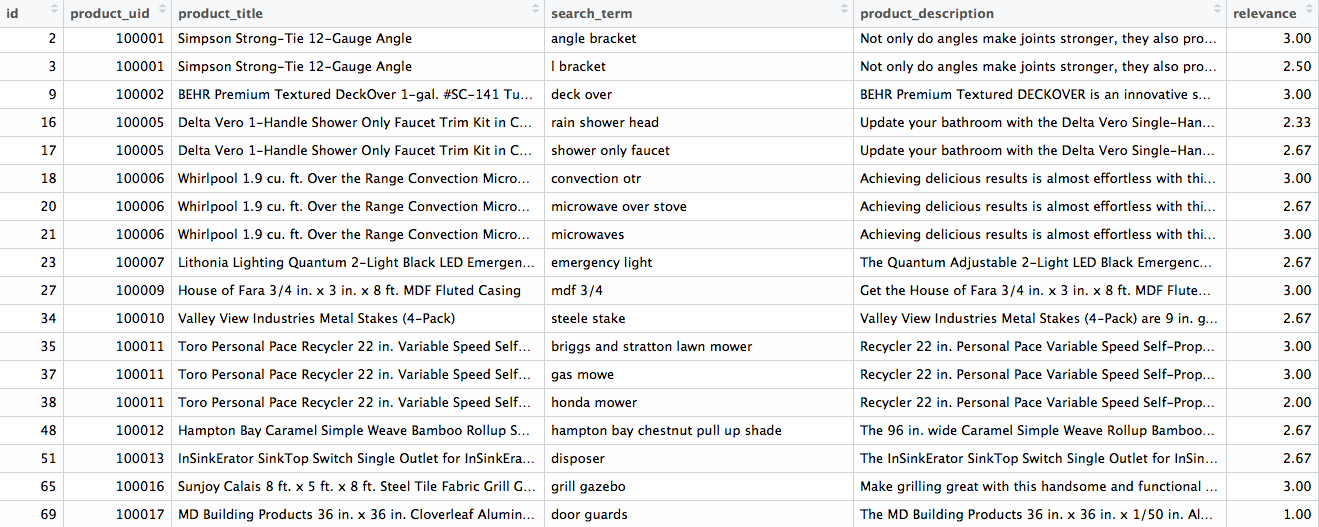
\includegraphics[width=3.5in]{raw_data} 
\caption{74067 observations}\label{fig:1} 
\end{figure} 
\subsection{Word Replacement}
By exploring the provided data, it seems important to perform some word replacements/alignments, e.g., spelling correction and synonym replacement, to align those words with the same or similar meaning.
\begin{figure}[htbp] 
\centering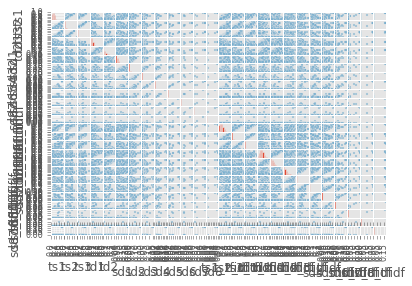
\includegraphics[width=3.5in]{download} 
\caption{Relevance}\label{fig:2} 
\end{figure} 
\subsubsection{Spelling Correction}
We just fixed the typo like "helloWorld" to "hello World", which seperated two individual word. What is more, we delete the stop words like "the", "and", for these words don't lend any support to our training.
\subsubsection{Synonym Replacement}
We replaced the synonym to reduce and simplify our data size.
\subsubsection{Other Replacements}
Including but not limited to removing insignificant punctuation like "\# , .", translating plurality like "feet" to "foot".
\begin{figure}[htbp] 
\centering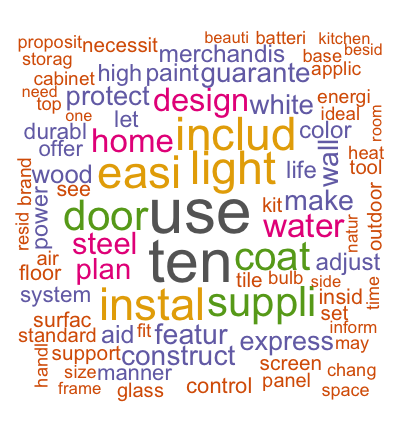
\includegraphics[width=3.5in]{CombineList} 
\caption{Combined List}\label{fig:3} 
\end{figure} 
\section{Feature Extraction/Selection}
We use function ngram(s, n) to extract string/sentence s’s n-gram (splitted by whitespace), where n = 1, 2, 3....

For example ngram(big red apple, 2) = [big red, red apple].

All the features are extracted for each run (i.e., repeated time) and fold(used in cross-validation and ensembling), and for the entire training and testing set (used in final model building and generating submission).
\subsection{Counting Features}
We generate counting features by calculating the total number of words in product title and search term. 

For some search terms, it only contains one word, like some ambiguous word ‘car’ or some meaningless stopword ‘to’, ‘or’. While there are still many meaningful one-word search term, multi-word search items are more likely to be specific and clear. 

Another counting features are the number of digits appeared in the product title and search term.
\begin{figure}[htbp] 
\centering\includegraphics[width=3.5in]{image1} 
\caption{Counting Features}\label{fig:4} 
\end{figure} 
\subsection{Jaccard Distance}
\begin{figure}[htbp] 
\centering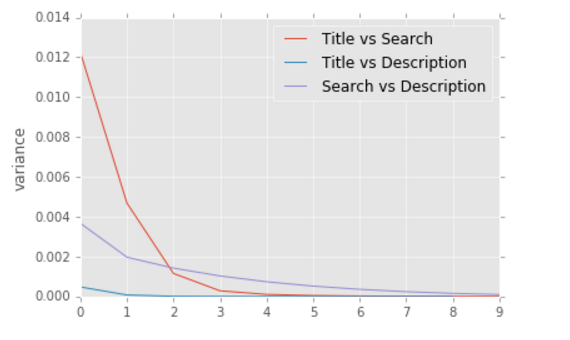
\includegraphics[width=3.5in]{dfeatures} 
\caption{Distance Feature}\label{fig:5} 
\end{figure} 
JaccardCoef(A,B) = $|A\bigcap B|/|A\bigcup B|$
We calculated the distance between "Search Item", "Product Description" and "Product Title" respectively. We thought it was important to compute the distance between "Product Description" and "Product Title" because ...
We tried many "n"s for our results, and found the optimal "n"s, n=3 for Product Title and Search Item, n=2 for Product Title and Product Description, n=8 for Search Item and Product Description.
\begin{figure}[htbp] 
\centering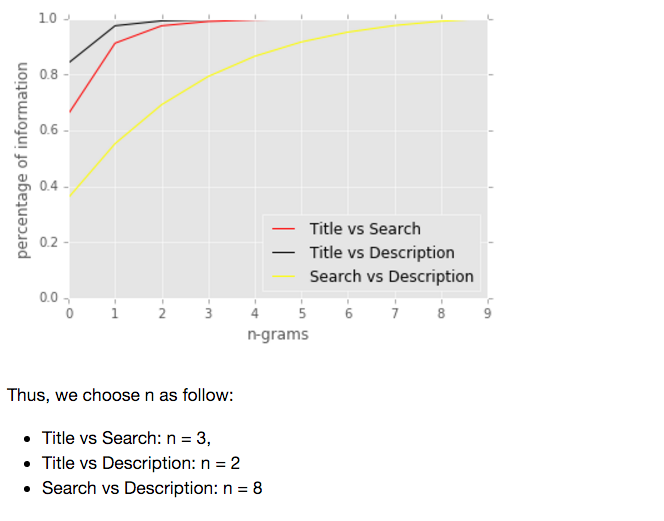
\includegraphics[width=3.5in]{dfeatures2} 
\caption{n-gram for Distance Feature}\label{fig:6} 
\end{figure} 
\subsection{Cosine Similarity with tf-idf}
\begin{figure}[htbp] 
\centering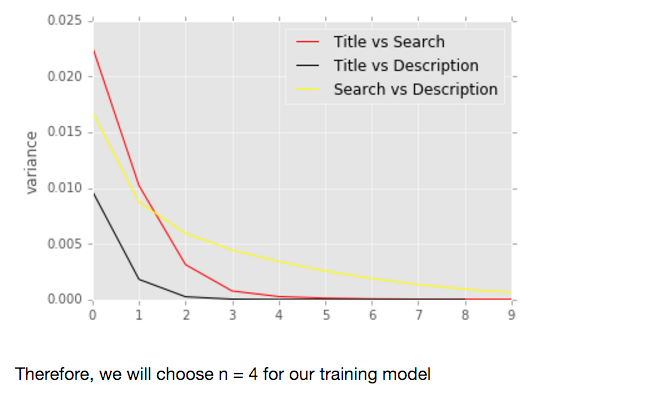
\includegraphics[width=3.5in]{tfidf} 
\caption{TF-IDF Feature}\label{fig:7} 
\end{figure} 
In the case of the term frequency tf(t,d), the simplest choice is to use the raw frequency of a term in a document. The inverse document frequency is a measure of how much information the word provides, that is, whether the term is common or rare across all documents.
\begin{figure}[htbp] 
\centering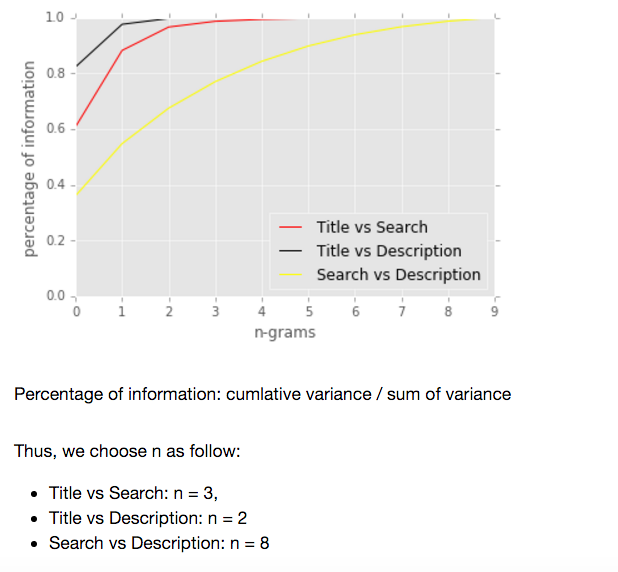
\includegraphics[width=3.5in]{tfidf2} 
\caption{n-gram for TF-IDF Feature}\label{fig:8} 
\end{figure} 
For n-gram selection of tf-idf, we have the similar result as Jaccard Coefficient distance.
\newpage
\subsection{Customized Features}
As most of items have their attributes in data, we choose the most three common attributes among products, brand, color and material. In these features, we used the method the same as Jaccard coefficient. Obviously, as many items only have one word in their color and material description, we would prefer 1-gram here.
\subsection{Combined Features}
Combined all the features above as our predictors.
\begin{figure}[htbp] 
\centering\includegraphics[width=3.5in]{image2} 
\caption{Combined Features}\label{fig:9} 
\end{figure} 
\section{Regression Analysis}
Because we found the relevance scores in training set are 1, 1.33, 1.5, 1.67, 2, 2.33, 2.5, 2.67. 3, we think regression should be better than classification.

For each model selection method, we use 5-fold cross-validation to avoid overfitting problem. The training data is broken up into 5 sections called ‘folds. At each iteration, we hide one fold and train the selected model on the remaining 4 folds. Grid search is applied to find several possible costs for most models. For each cost we quantify the model’s performance by taking the average test error over all folds, then pick the cost parameters with the lowest overall test error.
\subsection{Simple Linear Regression}
\begin{itemize}
\item{The basic understanding of relationship}
\item{Try as a starting point}
\end{itemize}
\subsection{Ridge Regression}
\begin{itemize}
\item{Alleciate multicollinearity among predictor variables}
\item{Grid-search to find optimal penalty}
\item{Search Range:} \\
Alpha:     $10e^{-6}$ to $10e^{-2}$
\end{itemize}
\subsection{Random Forest}
Random forest is a substantial modification that builds a large collection of de-correlated trees and then averages them. It is a popular ensemble selection method as the performance of random forest is very similar to boosting and corresponding parameters are simpler to train and tune.
\begin{itemize}
\item{Parameters range for grid-search:} \\
Number of trees in forest: 10-35 \\
Maximum depth of tree: 2-20
\end{itemize}
The final output shows that the optimal number of trees in forest is 33 and the maximum depth of tree is 10.
\subsection{Extreme Gradient Boosting}
XGBoost, short for ‘Extreme Gradient Boosting’, is also a ensemble model for supervised learning problem. It applies a more regularized model formalization to control over-fitting, which often gives a better performance. 
\begin{itemize}
\item{Search Range:} \\
Number of tree depth for base learners: 2-20\\
Number 10-35
\end{itemize}
The final output shows that the optimal number of tree depth is 9 and number of boosted trees to fit is 31.
\subsection{Neural Network Regressor}
\begin{figure}[htbp] 
\centering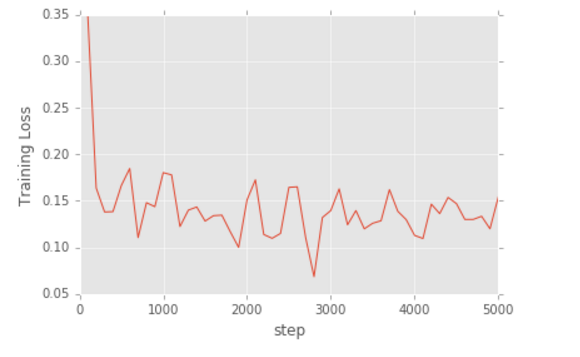
\includegraphics[width=3.5in]{nn_loss} 
\caption{Neural Network Loss}\label{fig:10} 
\end{figure} 
\begin{itemize}
\item{Layers: 4}
\item{Nodes: 50/layers}
\item{Steps: 5000}
\end{itemize}
\section{Conclusion}
We applied 5-folds cross validation for each regressors to generated the following table:


\ifCLASSOPTIONcaptionsoff
  \newpage
\fi




\begin{thebibliography}{1}

\bibitem{IEEEhowto:kopka1}https://github.com/tensorflow/skflow
\bibitem{IEEEhowto:kopka2}https://github.com/ChenglongChen/Kaggle\_CrowdFlower
\bibitem{IEEEhowto:kopka3}https://github.com/dmlc/xgboost

\end{thebibliography}







\end{document}


